%!TEX TS-program = xelatex
\documentclass[]{friggeri-cv}
\usepackage{afterpage}
\usepackage{hyperref}
\usepackage{color}
\usepackage{xcolor}
\hypersetup{
    pdftitle={},
    pdfauthor={},
    pdfsubject={},
    pdfkeywords={},
    colorlinks=false,       % no lik border color
   allbordercolors=white    % white border color for all
}
\addbibresource{bibliography.bib}
\RequirePackage{xcolor}
\definecolor{pblue}{HTML}{0395DE}

\begin{document}
\header{Tyler }{ Lyle}
      {Software Developer}
      
% Fake text to add separator      
\fcolorbox{white}{gray}{\parbox{\dimexpr\textwidth-2\fboxsep-2\fboxrule}{%
.....
}}

% In the aside, each new line forces a line break
\begin{aside}
  \section{Address}
    2115 New Road
    Waterford, PA 16441
    ~
  \section{Telephone}
    +1 (814) 464 3068
    ~
  \section{Mail}
    \href{mailto:}{\textbf{jobsearch\_lylet@}\\yahoo.com}
    ~
  \section{Web \& Git}
    \href{https://tyler-lyle.netlify.com/}{tyler-lyle.netlify.com}
    \href{https://bitbucket.org/tylerlyle}{bitbucket.org/\textbf{tylerlyle}}
    \href{https://github.com/lylet-AC}{github.com/\textbf{lylet-AC}}
    ~
  \section{Programming}
    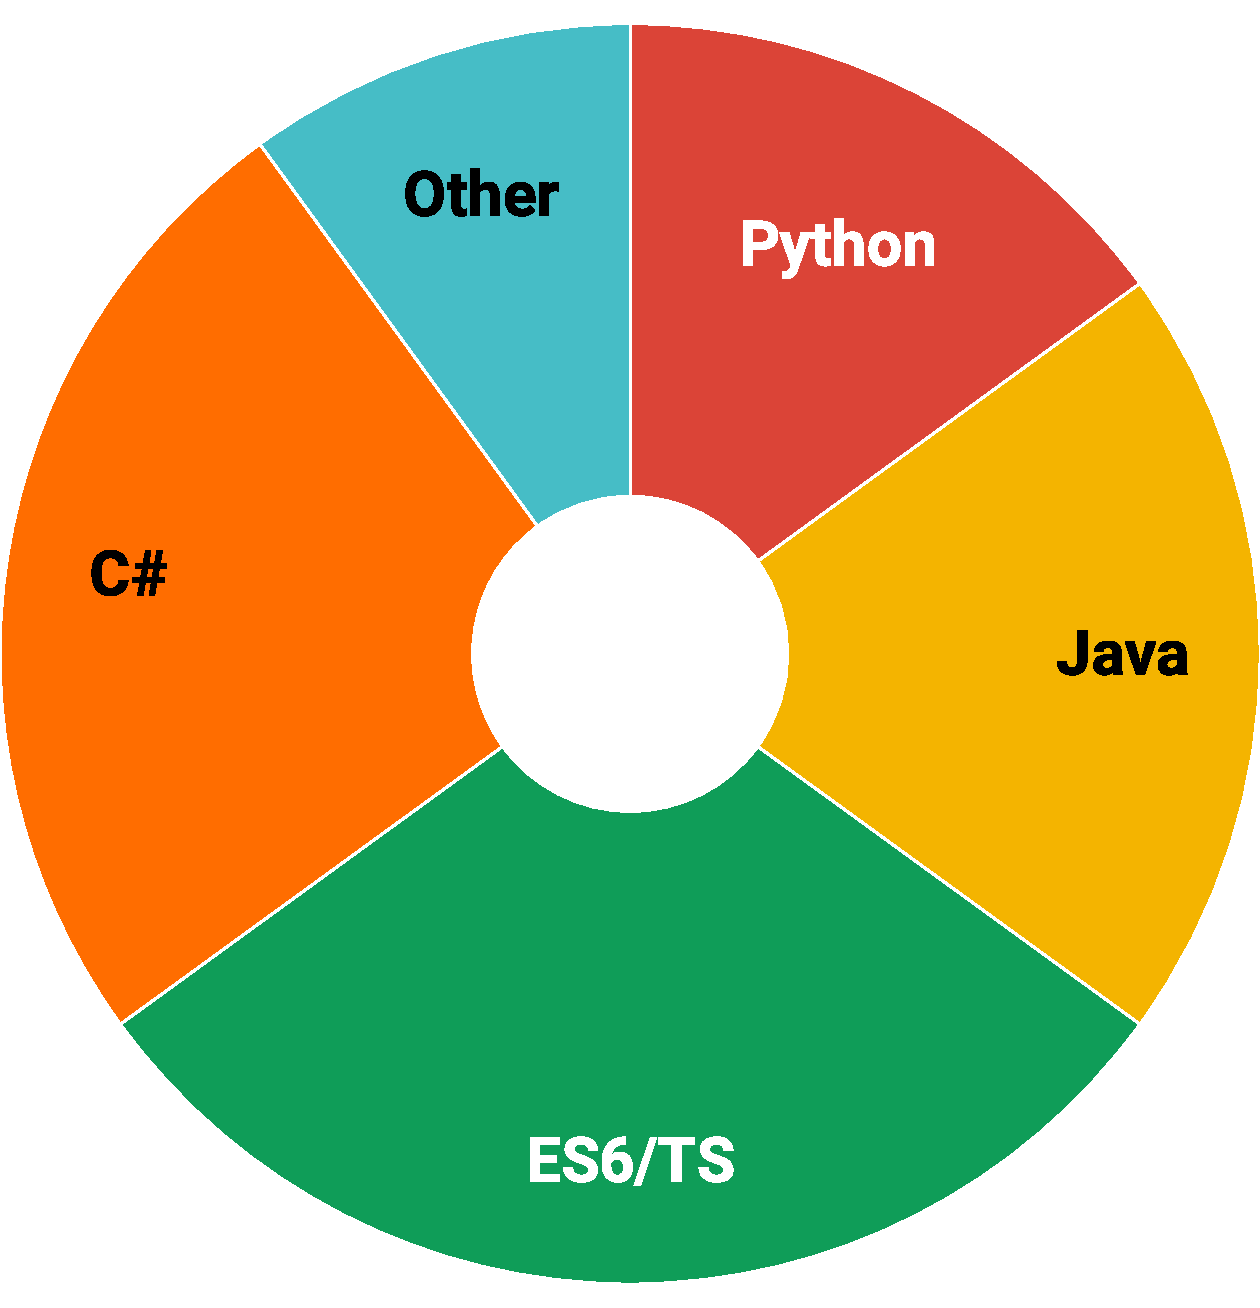
\includegraphics[scale=0.18]{img/pvl.pdf}
    ~
  \section{OS Preference}
    \textbf{GNU/Linux}
\includegraphics[scale=0.40]{img/5stars.png}
    \textbf{MacOS}
\includegraphics[scale=0.40]{img/3stars.png}
    \textbf{Windows}
\includegraphics[scale=0.40]{img/5stars.png}
    ~
  \section{Personal Skills}
    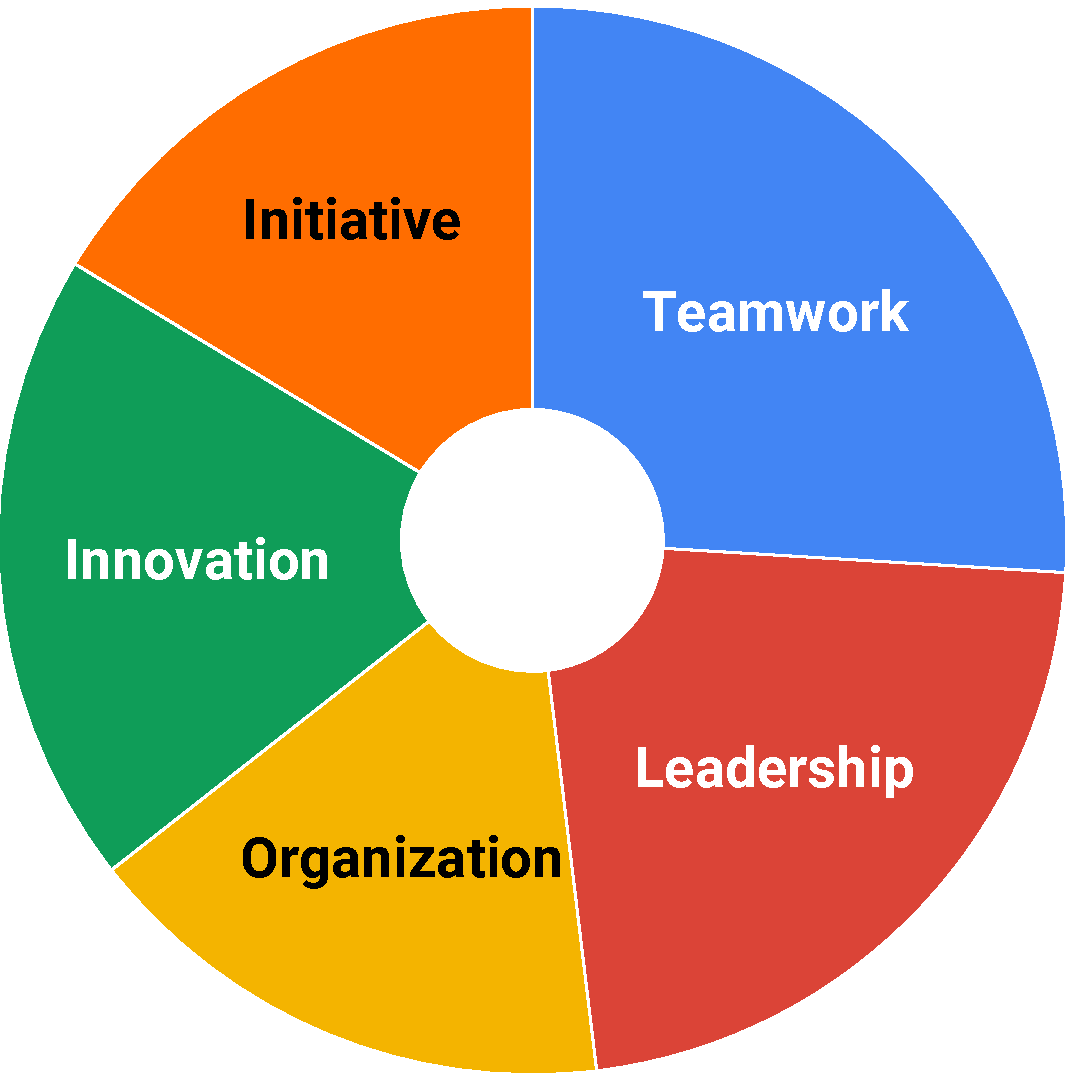
\includegraphics[scale=0.18]{img/skills.pdf}
    ~
\end{aside}

\section{About Me}
\begin{entrylist}
	\entry
	{}
	{Computer Enthusiast}
	{First Generation College Student}
	{
		I always have had a fascination with computing. Whether it be creating small websites at a young age to building fully featured applications now, I have always had a passion for development!  My love for computing doesn't just stop at the software level either.  As a hobby, I also build computers, host servers, and much more.  Computing, to me, is less a career and more a way of life.

	}
\end{entrylist}

\section{Education}
\begin{entrylist}
	\entry
	{2015 - 2019}
	{Bachelor's Degree in Computer Science}
	{Allegheny College}
	{Software Engineering.\\
		Main subjects: Software Engineering, Artificial Intelligence, Distributed Cloud Systems, Web Development.\\
	}

\end{entrylist}

\section{Software Projects}
\begin{entrylist}
	\entry
	{}
	{GatorGrader}
	{Allegheny College}
	{Python tool for the automated grading of Computer Science projects hosted on GitHub. \emph{Relator: Dr. Gregory Kapfhammer.}\\}
	
	\entry
	{}
	{Ardbot}
	{Allegheny College}
	{A multi-state robotic client designed for the autonomous playing of the popular e-sport game Rocket League. \emph{Relators: Prof. Janyl Jumadinova.}\\}
	
	\entry
	{}
	{Personal Website}
	{Personal Work}
	{My personal website developed using Angular 9 and deployed with Netlify. Check it out \underline{\href{https://tyler-lyle.netlify.com/}{here!}}\\}
	
\end{entrylist}

\section{Work Experience}
\begin{entrylist}
  \entry
    {8/19 - Now}
    {MIS / Jr. Programmer}
    {Expivia Marketing Interactions}
    {Used AngularJS and Angular coupled with .NET framework to build a REST API and multiple web apps.  Became familiar with SQL Server and setting up databases, tables, and entities.  Used an Object-Relational Mapper (ORM) to manage SQL entities in the .NET backend.  Experienced in using package managers and Angular CLI to kickstart new projects very quickly. Also gained experience with CSS layouts such as Flexbox and Grid.\\}
  \entry
    {6/13 - 2/18}
    {Shift Supervisor \& Closing Manager}
    {The Wendy's Company}
    {Ensure that food meets safety and quality standards, conduct interviews, train crew members, evening cash management, nightly inventory audits, establish goals.\\}
\end{entrylist}

\begin{flushleft}
\emph{January 5th, 2021}
\end{flushleft}
\begin{flushright}
\emph{Tyler Lyle}
\end{flushright}

\end{document}
